\chapter{Uygulama Onarım Rehberi}

\section{Sayfa ve Panel Onarım Rehberi}

\begin{warningbox}
\textbf{\faExclamationTriangle\ Yenile Sayfası Kaybolduysa veya Silindiyse}

\vspace{0.2cm}
Sistem dinamik panel mimarisine sahiptir. Sayfa silindiğinde sıfırlama yapmadan önce kodların varlığını doğrulamak yeterlidir.

\textbf{Adım Adım Onarım Süreci:}
\begin{enumerate}\setlength{\itemsep}{1pt}
    \item \textbf{Kod Varlığını Doğrulayın:} \textbf{\texttt{Alt + F11}} ile VBA editörüne girip modüllerin (\texttt{mod\_*}) sol menüde yer aldığını teyit edin.
    \item \textbf{Yeni Sayfa Açın:} Excel arayüzünde \textbf{"Yenile"} adında yeni ve boş bir çalışma sayfası oluşturun.
    \item \textbf{Kaydedip Çıkın:} Dosyayı kaydedip kapatın. Yeniden açtığınızda otomasyon motoru yeni sayfayı algılayacak ve panelleri otomatik çizecektir.
\end{enumerate}
\end{warningbox}

\begin{infobox}
\textbf{\faDatabase\ ARIZA, BAKIM veya GECENAY Sayfaları Kaybolduysa}

\vspace{0.2cm}
Veritabanı sayfalarından biri silindiyse veya adı bozulduysa:
\begin{enumerate}\setlength{\itemsep}{1pt}
    \item Silinen sayfanın ismiyle (\texttt{ARIZA}, \texttt{BAKIM} veya \texttt{GECENAY}) birebir eşleşen yeni bir çalışma sayfası oluşturun.
    \item Takip eden sayfadaki \textbf{Ekran Görüntüsü Referanslarını} inceleyerek tablo ve sütun yapısını orijinal haline getirin.
    \item Sayfanın 1. satırına takip edilen tarihleri \texttt{dd.mm.yyyy} formatında ekleyin.
    \item Dosyayı kaydedip kapatın. Sistem bir sonraki açılışta veritabanı adreslerini bu sayfa üzerinden yeniden haritalayacaktır.
\end{enumerate}
\end{infobox}

\section{Tarih ve Dönem Yönetimi}

\begin{infobox}
\textbf{\faCalendar*\ Yeni Tarih Tanımlama Mantığı}

\vspace{0.2cm}
Sistem dinamik kesişim algoritması (\texttt{FindIntersectCell}) kullandığı için VBA kodlarında tarih güncellemesi yapmanıza gerek yoktur. \texttt{ARIZA} veya \texttt{BAKIM} sayfalarının 1. satırını yeni tarihlerle \texttt{dd.mm.yyyy} formatında değiştirmeniz yeterlidir.
\end{infobox}


% ==========================================
% 3 RESMİN TEK SAYFADA TOPLANDIĞI BÖLÜM
% ==========================================
\newpage
\section{Veritabanı Sayfa Yapıları ve Görsel Referanslar}

\begin{warningbox}
\textbf{\faExclamationCircle\ Sütun Doğruluğu, İsimler ve Hücre İçeriği Uyarısı}

\vspace{0.2cm}
Sayfalar yeniden oluşturulurken aşağıdaki kurallara \textbf{özellikle dikkat ediniz}:
\begin{itemize}\setlength{\itemsep}{1pt}
    \item Personel/Vaka \textbf{İsimlerinin B sütununda} (\texttt{B} kolonu) yazılması gerektiğini unutmayınız.
    \item \textbf{''AÇIK VAKA SAYISI''} ve \textbf{''KAPALI VAKA SAYISI''} başlıklarının bulunduğu sütunların harf doğruluğuna, hizalamasına ve hücre içeriklerine azami özen gösteriniz.
    \item Hatalı sütun veya isim yerleşimi arka plan servislerinin yanlış adreslere veri yazmasına veya kayıtları bulamamasına neden olur.
\end{itemize}
\end{warningbox}

\vspace{0.2cm}

\begin{figure}[htbp]
    \centering
    % 1. Resim: ARIZA
    \fboxsep=0pt
    \fboxrule=0.6pt
    \fcolorbox{bordergray}{white}{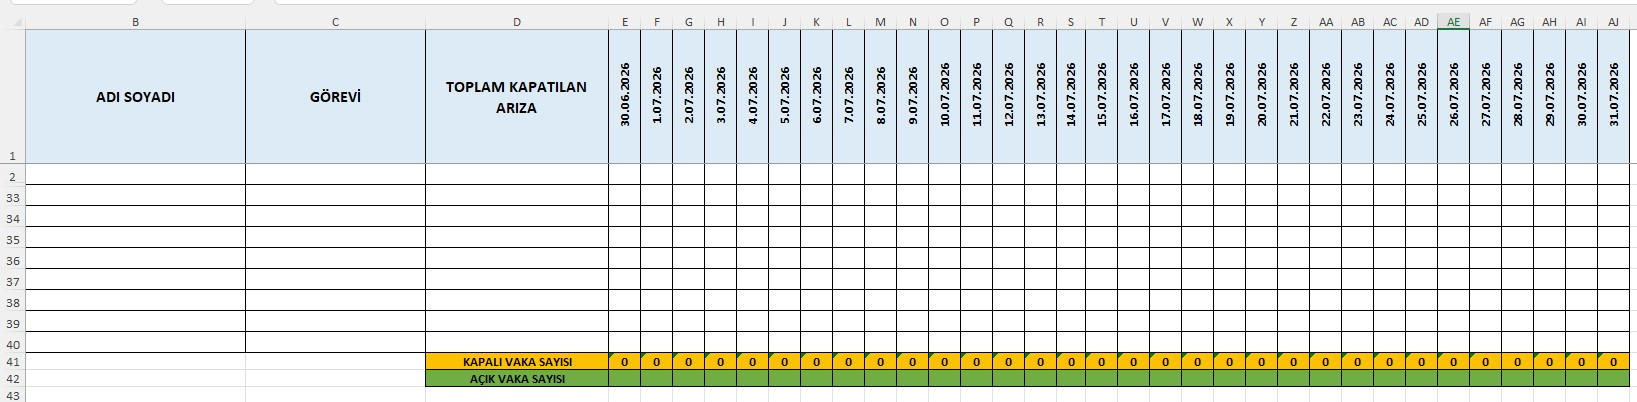
\includegraphics[width=0.92\textwidth, height=5.2cm, keepaspectratio]{ARIZA.jpg}}
    \caption*{ARIZA Sayfası Standart Tablo Yapısı (İsimler B Sütununda)}
    
    \vspace{0.2cm}
    
    % 2. Resim: BAKIM
    \fboxsep=0pt
    \fboxrule=0.6pt
    \fcolorbox{bordergray}{white}{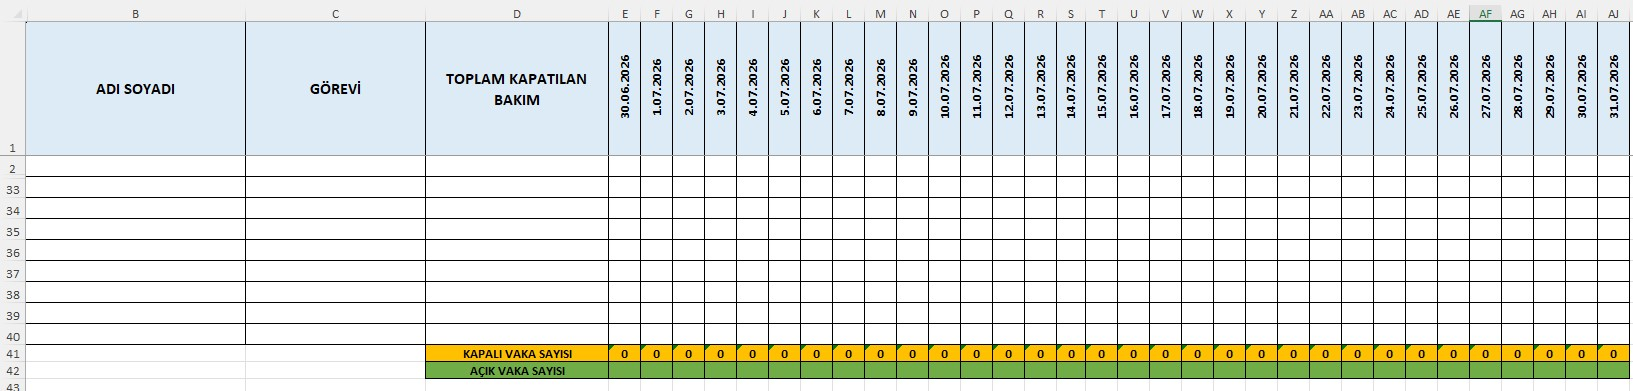
\includegraphics[width=0.92\textwidth, height=5.2cm, keepaspectratio]{BAKIM.jpg}}
    \caption*{BAKIM Sayfası Standart Tablo Yapısı (İsimler B Sütununda)}
    
    \vspace{0.2cm}
    
    % 3. Resim: GECENAY
    \fboxsep=0pt
    \fboxrule=0.6pt
    \fcolorbox{bordergray}{white}{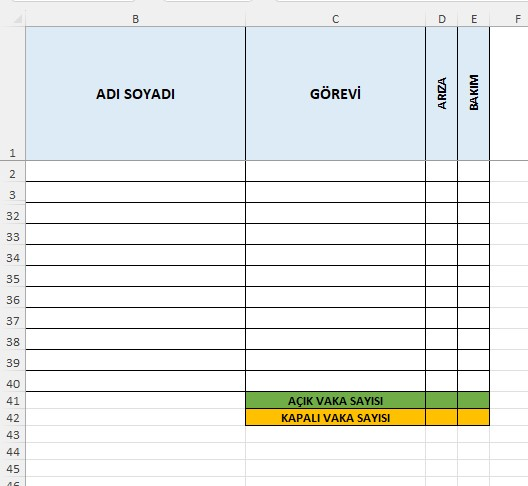
\includegraphics[width=0.92\textwidth, height=5.2cm, keepaspectratio]{GECENAY.jpg}}
    \caption*{GECENAY Sayfası Standart Tablo Yapısı (İsimler B Sütununda)}
    
    \caption{Veritabanı Sayfaları Standart Tablo Düzenleri (ARIZA, BAKIM, GECENAY)}
    \label{fig:all_db_sheets}
\end{figure}